%%\vspace{-5pt}
\section{Software Support for Peripheral Recovering} \label{sec:offline}
%%\vspace{-5pt}
%
With the enhanced NVP, REMARK will process the original program with the offline program transformer to pre-set safe checkpoints, collaborate with the new hardware modules and ensure realize efficient and reliable peripheral recovering and restarting.

\subsection{Peripheral Recover \& SCCP}	\label{sec:offlinePeriRec}
%
Recovering a peripheral is to restore the configuration states to its internal registers.
As is discussed in Sec.~\ref{sec:motivation}, neither software-based~\cite{jayakumar2014quickrecall} nor hardware-based~\cite{li2016hw} 'load-and-backup' recovering approach is usable in TPC.
Therefore, REMARK proposes a state tracking and `init-used' strategy that realizes lightweight, efficient peripheral recovery.

\noindent\textbf{Peripheral State Tracking.} \\
%
During system execution, the configuration of a peripheral is dynamically updated. 
Different from the 'load-and-backup' recovering approach, REMARK establishes a \textbf{configuration function queue (CFQ)} for each peripheral to track the usage of the configuration instructions, including the initialization instructions, along the execution and record the configuration states in PSRs.. 
Every time a new configuration instruction is executed, CFQ will be updated to include the latest configuration modification by a pre-inserted \emph{\_updateCFQ()} function.
Fig.~\ref{fig:updateCFQ} (a) shows the program where peripheral \emph{P1} is configured by \emph{\_P1\_configN()}.
To record this configuration, \emph{\_updateCFQ()} function is added after \emph{\_P1\_configN()}.
Fig.~\ref{fig:updateCFQ} (b) shows the pseudo code of \emph{\_updateCFQ()}.
\emph{\_updateCFQ()} can either update the parameters of an existing configuration function or add the new configuration function into CFQ.
In this way, new configurations to an existing status will not expand the capacity of CFQ and PSR.

%
\begin{figure}[t]
    \centering
    %\vspace{0pt}
    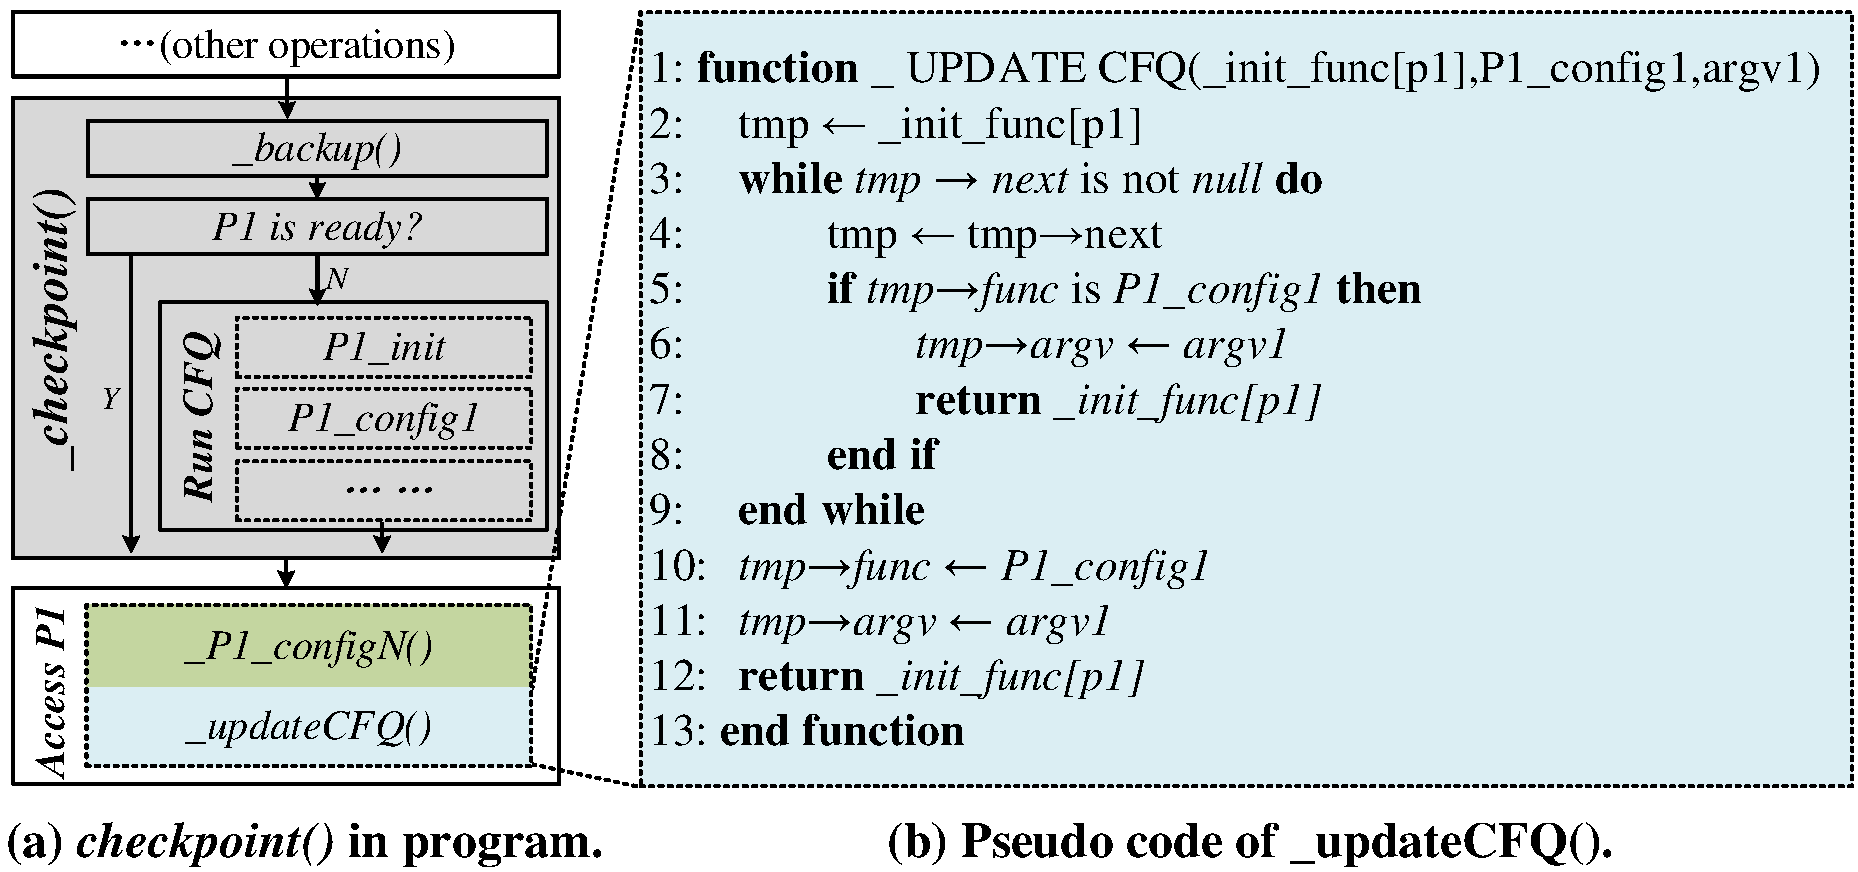
\includegraphics[width=0.48\textwidth]{Fig9_updateCFQ.pdf}
    %\vspace{-15pt}
    \caption{Program when peripheral \emph{P1} is accessed. \emph{\_checkpoint()} is used to configure \emph{P1} and \emph{\_updateCFQ()} is used to track the latest configurations.}
    %\vspace{-5pt}
    \label{fig:updateCFQ}
\end{figure}

\noindent\textbf{`Initi-used' Reconfiguration Strategy \& SCCP.} \\
%
A peripheral is ready to be called only if it is well configured.
Previous works~\cite{jayakumar2014quickrecall,li2016hw} has to `init-all' the peripherals after power failures in case of subsequent usages. 
However, if power failure occurs frequently, it leads to large reconfigurations overheads to `init-all' the peripherals.
To reduce the large reconfiguration overheads, REMARK provides an `init-used' approach, that is, instead of reconfiguring all the peripherals, we only need to reconfigure a peripheral whenever it is accessed. 
To realizes this strategy, REMARK needs to place a reconfiguration function before each peripheral functions.
Considering that the hybrid checkpointing strategy also requires to place SCCPs at the same place, we combine the reconfiguration function with the checkpointing function.

%
A \textbf{checkpoint function}, \emph{\_checkpoint()}, is inserted before each I/O operation to realize both the checkpointing and the reconfiguration functions.
With \emph{\_checkpoint()}, the processor rolls back to reconfigure the peripherals to avoid inconsistency.
Fig.~\ref{fig:updateCFQ} (a) shows the program where the checkpoint function, \emph{\_checkpoint()}, is inserted before the accesses of \emph{P1}.
\emph{\_checkpoint()} includes two parts: a backup function and a peripheral configuration part.
The backup function places a checkpoint before the I/O instruction in case of power failures.
Then, the program checks whether \emph{P1} is ready according to PSRs.
If \emph{P1} is not ready, the program will configure \emph{P1} with the configurations in CFQ.
Otherwise, the program skips the configuration part.
In this way, the `init-used' approach configures a peripheral only before it is invoked.


\subsection{Peripheral Restart \& SSCP}	\label{sec:offlinePeriRes}
%
When power failure crashes a peripheral operation, the system has to restart this uncompleted peripheral operation to avoid peripheral failures.
REMARK restart the uncompleted peripheral operations from SSCPs with the help of an initiator and PRM.

%\vspace{5pt}
\noindent\textbf{Initiator \& SSCP Pre-placement.} \\
%
REMARK proposes an \textbf{initiator} executed after power recovery to manage the recovery and restart of both the processor and the peripheral operations.
Its work flow is shown in Fig.~\ref{fig:InitiatorFlow}.
After the system is powered on, Bootstrap selects whether to enter the restart procedure or to start the program from the very beginning according to the \emph{$1^{st}\_start$} signal.
\emph{$1^{st}\_start$} is an external signal set by users.
If \emph{$1^{st}\_start$} is set, the processor is started from the very beginning.
Otherwise, initiator is started to recover the peripherals and restore the processor.

%
\begin{figure}[t]
    \centering
    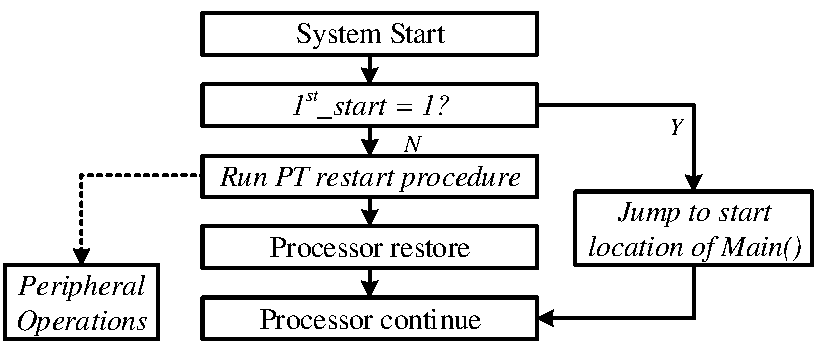
\includegraphics[width=0.48\textwidth]{Fig9_InitiatorFlow.pdf}
    %\vspace{-10pt}
    \caption{The working flow chart of initiator.}
    \label{fig:InitiatorFlow}
\end{figure}

As shown in Fig.~\ref{fig:Initiator}, initiator is a program located in the top of instruction memory used to store the peripheral checkpoints.
It contains a list of peripheral checkpoints and a processor restore instruction.
Each peripheral checkpoint is a restart function, \emph{\_restart\_PT()}, which can restart a specific peripheral operation.
The queue is empty at the beginning and is dynamically added by \emph{updateInitiator(ADD)} pre-placed after the peripheral operation starting functions.

%
An interrupt started by a peripheral indicates that the peripheral has completed its task and will enter idle mode.
The system does not need to restart a task if power fails after its completion.
To remove such invalid checkpoint, Initiator update function is inserted at the end of each ISR.
\emph{updateInitiator(REMOVE)} removes the peripheral checkpoint of the specific peripheral operation.

%
\begin{figure}[t]
    \centering
    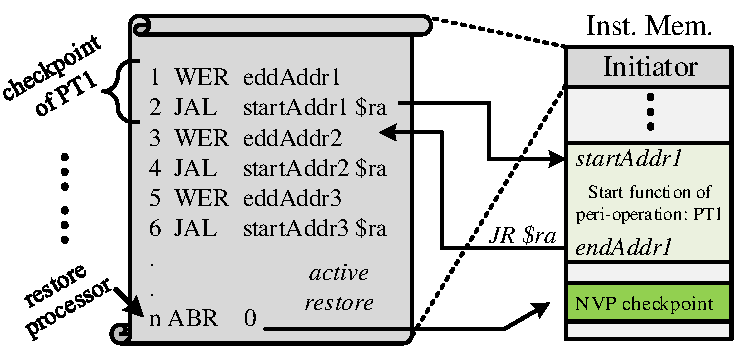
\includegraphics[width=0.48\textwidth]{Fig10_Initiator.pdf}
    %\vspace{-15pt}
    \caption{Restart peripheral operations in Initiator.}
    %\vspace{-1pt}
    \label{fig:Initiator}
\end{figure}

Each peripheral checkpoint consists of two instructions, \emph{WER} and \emph{JAL}.
Fig.~\ref{fig:Initiator} shows how to restart a peripheral operation, \emph{PT1}, with its checkpoint.
In this example, the first instruction writes the end address of \emph{PT1} start function, \emph{endAddr1}, into PRM.
The second instruction, \emph{JAL}, jumps to the start address of \emph{PT1} start function and links the address of the next instruction in Initiator into register \emph{\$ra}.
Then, the peripheral operation \emph{PT1} is restarted.
When the start function is finished, the PC counter reaches \emph{endAddr1}.
Then PRM automatically enable an \emph{JR \$ra} operation to return the program to Initiator and continue restarting the next peripheral operation.

%
%\vspace{5pt}
\noindent\textbf{Handle Hardware Interrupts.} \\
%
The ISR processing procedure requires safe checkpoints to avoid consistency problem.
Generally, an ISR should not be recovered, if it contains processor-peripheral interactions since the embedded volatile memory in a sensor loses all the data after power failure.
If the processor resumes the ISR, it will receive wrong data from the sensor which leads to system errors.
However, ISRs which contain no interactions can be safely recovered after power failure, such as a counter triggered by a timer.
To solve this application specific issue, REMARK provides a control bit, \emph{IR}, to the application developers to indicate whether an ISR can be restored according to application requirements.
Programmers can reset IR, if an ISR is recoverable, or set IR, if it's unrecoverable.
The IR is stored in IRec and the latter can set reliable checkpoints automatically during execution.

%
In this way, the program is transformed to be recoverable.
It is now ready to realize recoveries on the proposed hardware. 
Noted that, \emph{programmers can dictate an operation as unrecoverable by not using the wrapper codes according to application-specific reasons, such as data freshness requirements}.